\section{Data separability}
In addition to evaluate user performance in a real-time performance test, the clustering of the training data used to fit the classifier and regressors will be evaluated. 


\subsection{Principal Component Analysis}
PCA is used to express a set of possibly correlated variables into uncorrelated components, called principal components. A dataset of many variables can thus be expressed in a reduced dimensionality hyperspace using less variables that are the most defining for the given dataset. Each principal component (PC) is orthogonal on the former and are uncorrelated and have zero covariance. They each define the largest variance in an axis, such that PC 1 describes the direction of the maximum variance of the dataset. Each following PC describes the next highest variance of the dataset, with the constraint that is orthogonal and has zero covariance with any of the former PCs.
PCA is the orthogonal projection of data onto a lower dimension linear space. A PC is found by minimizing the variance by projecting the feature values (red dots) onto the line describing the highest variance in the data set (purple line) as seen on \figref{projection}. The PC (purple line) is found by minimizing the mean square distance between the data points. 

\begin{figure}[H] 
	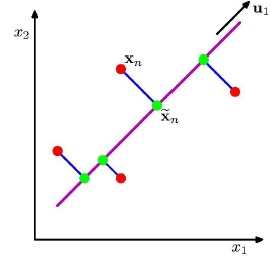
\includegraphics[width=0.3\textwidth]{figures/zASP/projection}
	\caption{Projection of data variables (red dots) onto PC axes (purple).}
	\label{projection}
\end{figure}
\vspace{-10pt}
The algebraic method of calculating the PCs can be done by using Singular Value Decomposition (SVD). The first step is to compute the squared cross product matrix of variances and covariances among every pair of the variables in the data set, where the diagonals are the variances and the off-diagonals are the covariances, as done in the following equation:
%\vspace{-20pt}
\begin{equation}
S = X \textquoteright X
\end{equation}
Where S is the cross product and X is the dataset matrix. When finding the PCs it includes an eigen-analysis of S. The eigenvalues of are solutions to the following equation:
%\verticalspace{1}
\begin{equation}
| S - \lambda I |  = 0
\end{equation}
Where $\lambda$ is the variances of each PC and I is the identity matrix. After solving for $\lambda$ the eigenvectors can be solved through the following equation:
\begin{equation}
det | S - \lambda I | b_{i} = 0
\end{equation}
Where $b_{i}$ is used to calculate the eigenvectors as in:
\begin{eqnarray}
u_{i} = \frac{b_{i}}{\sqrt{b_{i}^{\textquoteright} b_{i}}}
\end{eqnarray}
Where $u_{i}$ is the i number of eigenvectors that contain a contribution to the principal components.
The SVD orders the eigenvalues by size $\lambda_{1} > \lambda_{2} … > \lambda_{i}$. The scores for each PC is equal to the corresponding eigenvalue for that exact axis. The eigenvalues describe how much of the variance is accounted for by the associated PC. Summation of all eigenvalues accounts for the total variance of the data set; this is called the trace. To find how much the each PC accounts for, the eigenvalue of that PC is divided by the total variance: $\%~ of~ total~ variance~ = \frac{\lambda_{i}}{Trace}$. This can be used for deciding how many components are significant and by how much the dataset can be reduced. In our case this choice is made beforehand, due to the intention of visualizing the PCs in a three dimensional space. 